\documentclass[11pt, oneside]{article} 
\usepackage{geometry}
\geometry{letterpaper} 
\usepackage{graphicx}
	
\usepackage{amssymb}
\usepackage{amsmath}
\usepackage{parskip}
\usepackage{color}
\usepackage{hyperref}

\graphicspath{{figures/}{/Users/telliott/Github-Math/figures/}}
% \begin{center} \includegraphics [scale=0.4] {gauss3.png} \end{center}

\title{Archimedes' Quadrature (Lemma)}
\date{}

\begin{document}
\maketitle
\Large

%[my-super-duper-separator]
We verify one of Archimedes lemmas (propositions) very quickly.  

Let the parabola be $y=x^2$ with points $P=(v,v^2)$ and $Q=(u,u^2)$.  The secant $PQ$ has equation $y = (u+v)x - uv$ (check both points).  The tangent $QM$ has equation $y = 2ux - u^2$ (ditto).
\begin{center} 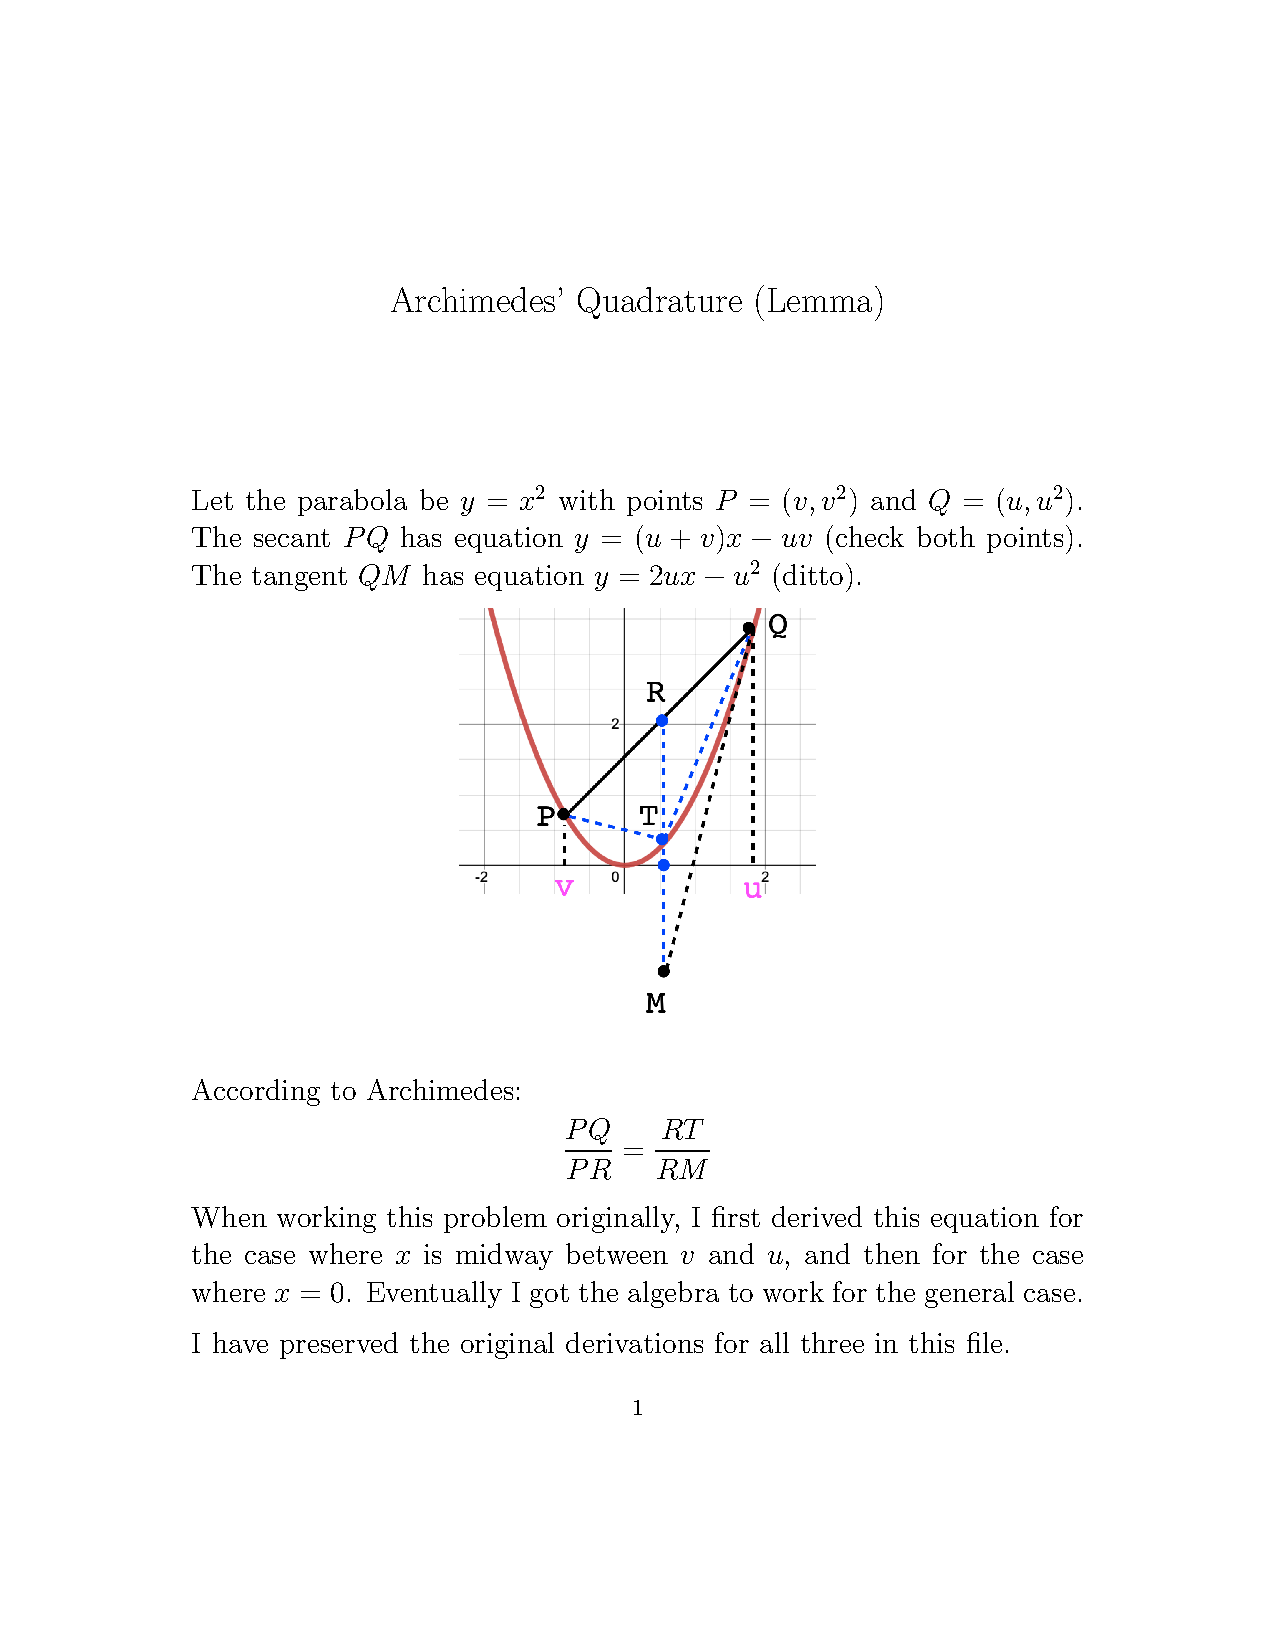
\includegraphics [scale=0.4] {qq3.png} \end{center}
So then let $w$ lie somewhere between $v$ and $u$, and then $T_y = w^2$.  We can get $R$ and $M$ from the equations above as $R_y = (u+v)w - uv$ and $M_y = 2uw - u^2$.

The first ratio is *
\[ \frac{PR}{PQ} = \frac{w-v}{u-v} \]
by similar triangles (bases and hypotenuses in same proportion).

Then the other ratio that we want to match it is $RT/RM$.
\[ |RT| = R_y - T_y = (u+v)w - uv - w^2 \]
\[ |RM| = R_y - M_y = (u+v)w - uv - 2uw + u^2 \]
\[ = vw - uv - uw + u^2 \]
We can be guided by the first ratio.  We want $(u-v)$ on the bottom.
\[ |RM| = u(u-v) + w(v - u) = (u-v)(u-w) \]
So then let's try to find $(u-w)$ on top
\[ |RT| =  (u+v)w - uv - w^2 \]
\[ = uw - uv + wv - w^2 \]
\[ = u(w - v) + w(v-w) = (u-w)(w-v) \]
Thus
\[ \frac{RT}{RM} = \frac{(u-w)(w-v)}{(u-v)(u-w)} = \frac{w-v}{u-v} = \frac{PR}{QR} \]
$\square$

* \emph{Proof} (additional).

The secant has equation $y = kx + y_0$ where $k = (u+v)$.  So $|RP|^2$
\[ = \Delta y^2 + \Delta x^2 = \ [ \ kw - y_0 - (k v - y_0) \ ]^2 + (w - v)^2 \]
\[ (k^2 + 1)(w - v)^2 \]
$|PQ|^2$ is exactly the same, with $u$ substituted for $w$.  So in the ratio of the square roots we have just $(w-v)/(u-v)$.

\end{document}